% Working document for the reply to Reviewer 1, comment 3 (and the
% "how much of the speed up is due to coordinate descent" sentence of the
% general remarks).
%
% 2026-10-27: added the Newton solver review before H1.
% Structure: Newton overview, then one section per hypothesis. Each gives the claim, the evidence
% so far, the objections a reviewer could raise, and the evidence still
% needed. H1-H4 are ours (2026-10-24); H5-H6 are proposed additions.
% Evidence paths are relative to reviews/.
% 2026-10-25: decomposition, H1-H5 and the accuracy sections updated with
% exp-017 (paper networks x gains 1-16 x all solvers, maxicao). Figures and
% tables: figures/exp017/; scripts: solvers/maxicao_matrix_20261024/
% (decompose.py, ratios.py, plot.py). The version before this update was
% not kept under Git.
%
% Compile: pdflatex r1_3_response.tex
\documentclass[11pt,a4paper]{article}
\usepackage[T1]{fontenc}
\usepackage[utf8]{inputenc}
\usepackage[margin=25mm]{geometry}
\usepackage{amsmath,amssymb}
\usepackage{xcolor}
\usepackage{booktabs}
\usepackage{tabularx}
\usepackage{enumitem}
\usepackage{graphicx}
\graphicspath{{figures/exp017/}{figures/reviews/exp017/}}
\usepackage[hidelinks]{hyperref}

\definecolor{responseblue}{RGB}{0,65,125}
\definecolor{todoorange}{RGB}{190,90,0}
\newenvironment{reviewercomment}
  {\begin{quote}\small\color{black}}
  {\end{quote}}
\newcommand{\todo}[1]{\textcolor{todoorange}{[TODO: #1]}}
\newcommand{\claim}[1]{\par\noindent\textbf{Claim.} #1\par}
\newcommand{\evidence}{\par\noindent\textbf{Evidence so far.}\par}
\newcommand{\objections}{\par\noindent\textbf{Objections a reviewer could raise.}\par}
\newcommand{\needed}{\par\noindent\textbf{Evidence still needed.}\par}
\newcommand{\decision}[1]{\par\noindent\textbf{Decision.} #1\par}
\setlength{\parindent}{0pt}
\setlength{\parskip}{0.6em}
\setlength{\emergencystretch}{2em}
\setlist{itemsep=0.2em, topsep=0.2em}

\title{Reply to Reviewer 1, comment 3: working document\\[0.5em]
\large Where does the speed-up over ELDO come from?}
\author{}
\date{Working draft, 27 October 2026}

\begin{document}
\maketitle

\section*{The question}

\begin{reviewercomment}
3. What is the algorithmic benefit of coordinate descent?

The authors primary result is a speedup v.s., a general-purpose commercial
SPICE solver. However, the root cause of this speedup is not established
in the paper. As an example, a reasonable baseline might be to solve the
KCLs with a purpose-built Newton, damped-Newton, or related sparse solver.
After all the authors already use Newton-Raphson for the PWL updates and
to solve their Lambert-w formulation.
\end{reviewercomment}

From the general remarks:

\begin{reviewercomment}
The comparison against a general-purpose SPICE simulator would have
benefited from greater analysis/isolation of confounders e.g., can we
quantify how much of the speed up is due to coordinate descent and how
much (if any) could be due to the use of a specialized equilibrium solver.
\end{reviewercomment}


% -------------------------------------------------------------------
% BEGIN NEWTON SOLVER REVIEW
% Integrated from newton_solvers_review.md, 27 October 2026.
% Variants 3--6 were excluded at the author's request.
\section*{Newton solvers: structure, implementation and evidence}

\subsection*{Summary}

Armijo-damped block-Cholesky Newton (N1) is the solver to defend in the reviewer
response, with dense-LU Newton as the baseline.

\begin{itemize}
\item It takes exactly the dense-LU steps at 4.6\ensuremath{\times} lower cost (geometric
mean, 2.0--104\ensuremath{\times}). It converged on all 52,200 exp-017 paper-network
solves.
\item Its weakness is the step count. That rises from 7.2 to 19.2 mean steps between
1\ensuremath{\times} and 16\ensuremath{\times} gain, because nothing limits the junction
overshoot.
\item As a result, adaptive CD (L3) overtakes it from about 4\ensuremath{\times} gain, and the
lean CD (LITE) beats it on 139 of 145 network--gain pairs.
\item Junction limiting and Newton--Krylov, the two variants that could change this picture,
are designed but not yet built.
\end{itemize}

\subsection*{Problem setting}

Every Newton variant solves the same DC equilibrium of the layered DRN: Kirchhoff's
current law at every free node, stacked into one system.

\[
F(v) = A v - f + i(v) = 0, \qquad J(v) = A + \operatorname{diag}\big(i'(v)\big)
\]

\begin{itemize}
\item \textbf{$A$} is block tridiagonal by layer. Its diagonal blocks are diagonal (no
connections inside a layer), with $2a=\operatorname{colsum}(W_l)+a_v
a_i\operatorname{rowsum}(W_{l+1})$. The off-diagonal blocks are $-a_iW$ above and
$-a_vW^{\mathsf T}$ below.
\item \textbf{$J$ is not symmetric} for the paper's amplifiers ($a_v=4,\ a_i=1$), but a fixed
layer scaling makes it symmetric positive definite. The next section derives this
structure and the three direct factorizations it permits.
\item \textbf{$f$} is the clamped input through $W_{0}$ on the first free layer. exp-017 has
no bias currents.
\item \textbf{$i(v)$} is the device law on hidden nodes only: full antiparallel double
Shockley ($I_s=1\,\mu\mathrm{A},\ V_T=50\,\mathrm{mV},\
V_{\mathrm{off}}=0.8\,\mathrm{V}$), or the oriented single Shockley for single\_* nets.
\end{itemize}

Size: $n$ = sum of free widths. Double nets have 20 outputs and single nets 10, so
double\_h2w1024 has $n=2068$.

\textbf{Stopping rules} shared by all variants (\nolinkurl{harness/solver.py}):

\begin{itemize}
\item current: $\max|F|\leq\mathrm{tol}$, in amperes. This is the primary stop in exp-017
(grid $10^{-2}$ to $10^{-10}$ A).
\item voltage: $\max|F/\operatorname{diag}(A)|\leq\mathrm{tol}$, in volts.
\item CD rule: $\max|\Delta v|\leq\mathrm{rtol}\max|v_{\mathrm{old}}|+\mathrm{atol}$ on the
accepted step, for like-for-like comparison with the repository CD.
\end{itemize}

All runs start from $v=0$ unless a linear-solution start is named. The Armijo merit
function is always the conductance-scaled 2-norm $\|F/\operatorname{diag}(A)\|_2$,
whichever stop is used.

\subsection*{Jacobian structure: dense LU, block LU, block Cholesky}

At each Newton iteration we solve $J(v)\Delta v=-F(v)$. Dense LU, block LU and block
Cholesky solve this same linear system; they differ in how much of its structure they
use. With exact arithmetic and the same step rule, they give the same Newton iterates.
Floating-point results can differ by roundoff.

Number the free layers $j=0,\ldots,h$: $h$ hidden layers followed by the output layer.
Let $w_{j}$ be their widths, $m=w_h$ the output width, and $n=\sum_{j=0}^{h}w_j$.
The input is clamped and is not an unknown. With $W_{0}$ connecting the input to layer 0
and $W_{j+1}$ connecting free layers $j$ and $j+1$, the Jacobian is

\[
J(v) =
\begin{bmatrix}
B_0 & E_0 & 0 & \cdots & 0 \\
C_0 & B_1 & E_1 & \ddots & \vdots \\
0 & C_1 & B_2 & \ddots & 0 \\
\vdots & \ddots & \ddots & \ddots & E_{h-1} \\
0 & \cdots & 0 & C_{h-1} & B_h
\end{bmatrix}.
\]
\[
E_j = -a_i W_{j+1}, \quad C_j = -a_v W_{j+1}^{\mathsf T},
\]

\[
B_j(v) = \operatorname{diag}\!\left[
\operatorname{colsum}(W_j)
+ a_v a_i\,\operatorname{rowsum}(W_{j+1})
+ g_j(v_j)\right],
\]
\[
g_j(v_j)=i'_j(v_j).
\]

At the output, the outgoing-weight term is absent and $g_h=0$. Every $B_{j}$ is
diagonal because there are no connections within a layer and each shunt depends only on
its own voltage. The adjacent-layer blocks are generally dense; all other blocks vanish.
Only $g_{j}$ changes during Newton, so the off-diagonal blocks and the sparsity pattern
stay fixed.

The distinction that matters for the solve is \textbf{diagonal before elimination,
generally dense after elimination}. Eliminating one layer couples the nodes of the next
through shared neighbours. Block methods retain those dense Schur complements while
avoiding a dense matrix for the whole network.

\subsubsection*{Dense LU: factor the full Jacobian}

Assemble the $n\times n$ matrix and factor it with partial row pivoting, $PJ=LU$, then
solve the two triangular systems for $\Delta v$. This is the general-matrix route used
by \nolinkurl{backend='dense_lu'}; it makes no use of the layer pattern or the
symmetrizing scale. Partial pivoting is the standard
\href{https://www.netlib.org/lapack/explore-html/db/d04/group__getrf_gaea332d65e208d833716b405ea2a1ab69.html}{LAPACK
DGETRF} factorization.

The leading factorization cost is $\frac{2}{3}n^3$ flops, with $O(n^2)$ storage and
$O(n^2)$ work for one right-hand side after factorization. For $h$ hidden layers of
width $w$, $n=hw+m$. Even with just one hidden layer, dense LU pays a cubic cost in $w$.

\subsubsection*{Block LU: eliminate one layer at a time}

Block LU uses the block-tridiagonal pattern directly on $J$. Write $r=-F(v)$, and
eliminate from the input side:

\[
T_0 = B_0, \qquad \widehat r_0 = r_0,
\]

\[
\begin{aligned}
T_j &= B_j - C_{j-1}T_{j-1}^{-1}E_{j-1},\\
\widehat r_j &= r_j - C_{j-1}T_{j-1}^{-1}\widehat r_{j-1}
\quad (j=1,\ldots,h).
\end{aligned}
\]

Then back-substitute from the output:

\[
\Delta v_h = T_h^{-1}\widehat r_h, \qquad
\Delta v_j = T_j^{-1}(\widehat r_j-E_j\Delta v_{j+1}).
\]

The inverse notation means linear solves; no inverse is formed. $T_{0}$ is diagonal, so
its solves are divisions. Later $T_{j}$ are generally dense and can be factored by LU,
reusing each factor for the coupling block and the residual. This is block Thomas
elimination by physical layer, distinct from the internal BLAS blocking used by a dense
LU routine.

For comparable layer widths, the work scales as $O(hw^3)$ and storage as $O(hw^2)$,
instead of dense LU's $O(h^3w^3)$ work and $O(h^2w^2)$ storage when $m$ is small. This
remains cubic in width. For h1, the stronger saving comes from the diagonal first block:
the only dense factorization is the $m\times m$ output Schur complement, giving
$O(wm^2+m^3)$ work.

For this DRN, the $T_{j}$ equal the positive-definite Schur blocks derived below, so
elimination does not require exchanging layers. A generic block-tridiagonal matrix
does not have that guarantee. \textbf{Block LU is a structural comparison here:}
\nolinkurl{LayeredDRN.linear_step()} currently exposes dense LU and block Cholesky, with
no separate block-LU backend or measured block-LU timings.

\subsubsection*{Block Cholesky: use the layer structure and symmetry}

The amplifier gains make $J$ nonsymmetric, but the asymmetry is fixed across Newton
steps. Define a diagonal scale that is constant within each layer:

\[
D = \operatorname{blockdiag}(D_0,\ldots,D_h),
\qquad D_j=(a_i/a_v)^{j/2}I_{w_j},
\qquad S = D J D^{-1}.
\]

The diagonal blocks remain $B_{j}$, while the upper and lower blocks become $K_j$ and
$K_j^{\mathsf T}$, with $K_j=-\sqrt{a_va_i}\,W_{j+1}$. Thus $S$ is symmetric. For $a_v$ =
4 and $a_i$ = 1, the layer scales are 1, 1/2, 1/4, \ldots{} . The equivalent Newton
system is

\[
S y = D r, \qquad y = D\Delta v, \qquad \Delta v = D^{-1}y.
\]

Positive definiteness follows from the network's quadratic form. Each conductance c
between free nodes p and q in consecutive layers contributes
$c(\sqrt{a_va_i}\,x_p-x_q)^2$; each connection to the clamped input contributes
$cx_q^2$; and each shunt contributes $g_px_p^2$. All are nonnegative for monotone
shunts. The sum is strictly positive for nonzero $x$ if every connected free component
is anchored by an input connection or a positive shunt derivative. The paper's connected
networks satisfy this condition; an unanchored component with zero shunt derivatives
would only give positive semidefiniteness.

Elimination therefore preserves positive definiteness:

\[
H_0 = B_0, \qquad
H_j = B_j-K_{j-1}^{\mathsf T}H_{j-1}^{-1}K_{j-1},
\qquad H_j=R_jR_j^{\mathsf T}.
\]

Use the same forward elimination and back-substitution as above, with $K^{\mathsf T}$,
$K$ and the scaled right-hand side $Dr$, then unscale the result. Since $D_j$ is a
scalar multiple of the identity within each layer, the block-LU $T_{j}$ and these
$H_{j}$ are equal in exact arithmetic. Block Cholesky exploits their symmetry and
positive definiteness when factoring them. The implementation is a block $LDL^{\mathsf
T}$ elimination with a Cholesky factorization of each dense Schur block;
\href{https://www.netlib.org/lapack/explore-html/d2/d09/group__potrf_ga84e90859b02139934b166e579dd211d4.html}{LAPACK
DPOTRF} supplies the SPD factorization without pivoting.

Factoring a dense $w_j\times w_j$ Schur block costs about $\frac{1}{3}w_j^3$ flops with
Cholesky, versus $\frac{2}{3}w_j^3$ with LU. Both block methods still pay for coupling
solves and Schur products, so this does not imply a twofold speedup of the whole solve.
The current code forms $K^{\mathsf T}(H^{-1}K)$ with a general matrix product. A
Cholesky implementation can instead use $Z=R^{-1}K$ and form $Z^{\mathsf T}Z$ with a
symmetric rank-k update; that optimization is not yet used here.

\begin{center}
\small
\setlength{\tabcolsep}{4pt}
\begin{tabularx}{\linewidth}{@{}p{0.15\linewidth}X p{0.22\linewidth}p{0.18\linewidth}@{}}
\toprule
Linear solve & Structure used & Work, $h\geq2$, $m\ll w$ & h1 work \\
\midrule
Dense LU & General nonsymmetric matrix & $O((hw+m)^3)$ & $O((w+m)^3)$ \\
\addlinespace
Block LU & Block tridiagonality and diagonal first block & $O(hw^3)$, for $h\geq2$ & $O(wm^2+m^3)$ \\
\addlinespace
Block Cholesky & Same layer structure, plus diagonal symmetrization and SPD Schur blocks & $O(hw^3)$, for $h\geq2$, with cheaper block factorizations & $O(wm^2+m^3)$ \\
\bottomrule
\end{tabularx}
\end{center}

The available backends are \texttt{dense\_lu} and \texttt{block\_cholesky}; block LU is a comparison only.

The large h1 saving comes from eliminating the diagonal hidden block and factoring only
the small output block. With h2/h3, elimination creates dense hidden-layer Schur
complements, and cubic work in the hidden width remains. These are linear-algebra
savings; they do not by themselves reduce Newton's iteration count.

\emph{Implementation reference: Jacobian assembly and linear solve
(\nolinkurl{reviews/solvers/solver.py:155}). The operation counts above describe
arithmetic scaling, not measured timings.}

\subsection*{What ELDO solves}

ELDO solves the same equilibrium, but in a larger formulation. Its unknowns include the
amplifiers' internal nodes and branch currents. Eliminating those exactly gives back
$J(v)$ above.

\textbf{Circuit.} The paper netlist builds each hidden neuron as a subcircuit with two
nodes, VIN and VOUT:

\begin{itemize}
\item the behavioural GEXP shunt diodes sit on VIN;
\item a VCVS imposes $V(\mathrm{VOUT})=a_vV(\mathrm{VIN})$;
\item a CCCS injects $a_i$ times the VCVS branch current back into VIN;
\item resistors connect each VOUT to the next layer's VIN nodes.
\end{itemize}

Output nodes are plain nodes. The inputs are grounded voltage sources
(VAC1\ldots{}VAC128, the signed-pair inputs times the gain), so ELDO eliminates them.

\textbf{Unknowns.} Modified nodal analysis (MNA) keeps three groups:

\begin{itemize}
\item $u$: VIN of every hidden neuron and the output nodes, which are the $n$ unknowns $v$ of
the local solver;
\item $y$: VOUT, one per hidden neuron;
\item $I$: the VCVS branch current, one per hidden neuron.
\end{itemize}

Each hidden neuron therefore carries three unknowns (VIN, VOUT, $I$) where the local
solver has one (VIN); output nodes carry one in both. That gives $N=n+2\sum_{j<h}w_j$
equations. These are ELDO's own equation counts, read from each run's
\nolinkurl{netlist.chi}:

\begin{center}
\small
\setlength{\tabcolsep}{4pt}
\begin{tabular}{@{}lrrr@{}}
\toprule
Net & ELDO equations & Local unknowns & Ratio \\
\midrule
h1w128 & 3\ensuremath{\cdot}128 + 20 = 404 & 148 & 2.7 \\
\addlinespace
h2w128 & 3\ensuremath{\cdot}256 + 20 = 788 & 276 & 2.9 \\
\addlinespace
h3w256 & 3\ensuremath{\cdot}768 + 20 = 2,324 & 788 & 2.9 \\
\addlinespace
h2w512 & 3\ensuremath{\cdot}1,024 + 20 = 3,092 & 1,044 & 3.0 \\
\bottomrule
\end{tabular}
\end{center}

The ratio stays slightly under 3 because the 10--20 output nodes count once on both
sides. It is 3 times as many unknowns, not 2: VIN and VOUT account for a factor of 2,
and the VCVS branch current $I$ for the third.

\textbf{Why ELDO carries $I$.} MNA builds its equations element by element, with one KCL
row per node. Each element adds ("stamps") its current into the rows of the nodes it
touches, and that current must be expressible in the unknowns:

\begin{center}
\small
\setlength{\tabcolsep}{4pt}
\begin{tabularx}{\linewidth}{@{}p{0.28\linewidth}X p{0.24\linewidth}@{}}
\toprule
Element & Current in terms of the unknowns & Extra unknown \\
\midrule
Resistor & $i=g(V_a-V_b)$: conductance entries & none \\
\addlinespace
Diode (each Newton iteration) & tangent conductance + current source & none \\
\addlinespace
Current-controlled current source & a known multiple of an existing unknown & none \\
\addlinespace
Voltage source, including the VCVS & not expressible & branch current $I$, plus one constraint row \\
\bottomrule
\end{tabularx}
\end{center}

A voltage source fixes a voltage, not a current. Its law, here
$V(\mathrm{VOUT})-a_vV(\mathrm{VIN})=0$, says nothing about the current it delivers. An
ideal source supplies whatever the load draws, so the current depends on the rest of the
circuit. MNA therefore adds the branch current $I$ as an unknown, which appears in the
VOUT KCL row, and the source's law as an extra row. These are the third block row and
the $I$ column of the matrix below.

In this circuit $I$ is needed a second time. The CCCS is a SPICE F element, and an F
element is controlled by the branch current of a voltage source, here the VCVS. $I$ must
exist as an unknown for the CCCS to refer to.

\textbf{Why the local solver can drop it and ELDO does not.} $I$ enters linearly. From
the VOUT row, it is the current flowing out through the resistors to the next layer:

\[
I = -\big(G_{yu}\,u + G_{yy}\,y\big).
\]

Substituting it, together with $V(\mathrm{VOUT})=a_vV(\mathrm{VIN})$, into the VIN rows
removes both unknowns. This is where the $a_va_i\operatorname{rowsum}(W)$ term and the
nonsymmetric off-diagonal blocks of $J$ come from. The local solver can do this because
every neuron has the same known structure. ELDO keeps the per-element stamps because
they work for any netlist. An ideal source would be an infinite conductance, so it
cannot be stamped as one. The extra rows are cheap per element, but here they add 2
unknowns per hidden neuron.

ELDO could avoid $I$ only with a different circuit. For example, the amplifier could be
modelled as a VCCS with a large output conductance (a Norton equivalent). That is no
longer an ideal VCVS, and the large conductance would worsen the matrix conditioning.
With the paper netlist, the third unknown is unavoidable.

\textbf{Newton system.} Every ELDO iteration replaces each diode by its tangent
conductance $g=i'(u)$ plus a current source, and solves

\[
\begin{bmatrix}
G_{uu} + \operatorname{diag}(g) & G_{uy} & -a_i P \\
G_{yu} & G_{yy} & \mathbb I \\
-a_v P^{\mathsf T} & \mathbb I & 0
\end{bmatrix}
\begin{bmatrix} \Delta u \\ \Delta y \\ \Delta I \end{bmatrix}
= -\begin{bmatrix} F_u \\ F_y \\ F_I \end{bmatrix}.
\]

Here $\mathbb I$ denotes an identity matrix, distinct from the branch-current vector $I$. The blocks are:

\begin{itemize}
\item $G_{uu}$: the incoming conductances, $\operatorname{colsum}(W_j)$, which form a
diagonal;
\item $G_{yy}$: the outgoing conductances, $\operatorname{rowsum}(W_{j+1})$, which also form a
diagonal;
\item $G_{uy}=G_{yu}^{\mathsf T}$: the $-W$ couplings from each VOUT to the next
layer's VIN;
\item $P$: the embedding matrix, so that $P^{\mathsf T}u$ selects the hidden nodes;
\item the third block row: the VCVS constraint;
\item the $-a_iP$ column: the CCCS.
\end{itemize}

\textbf{Reduction to $J$.} Eliminate $y$ and $I$, which appear linearly. Once their linear equations hold
($F_y=F_I=0$), the VCVS row gives $\Delta y=a_vP^{\mathsf T}\Delta u$, and the VOUT row then gives $\Delta I$.
Substituting both into the VIN row leaves

\[
\begin{aligned}
\big(&G_{uu} + \operatorname{diag}(g) + a_v a_i\,P G_{yy} P^{\mathsf T}\\
&{}+ a_v G_{uy} P^{\mathsf T} + a_i P G_{yu}\big)\,\Delta u = -F_u ,
\end{aligned}
\]

which is $J(v)$ term by term:

\begin{itemize}
\item $a_va_iPG_{yy}P^{\mathsf T}$ is the $a_va_i\operatorname{rowsum}(W_{j+1})$ part of
$B_{j}$;
\item $a_vG_{uy}P^{\mathsf T}$ is the lower block $C_j=-a_vW_{j+1}^{\mathsf T}$;
\item $a_iPG_{yu}$ is the upper block $E_j=-a_iW_{j+1}$.
\end{itemize}

\nolinkurl{eldo_linear_algebra_20261022} rebuilds this matrix from archived netlists,
and its equation and nonzero counts match ELDO's own. Its Schur complement reproduces
the MNA solve to \ensuremath{\leq} $2\times 10^{-14}$. The equations and the equilibrium
are therefore identical; the difference is in how each solver reaches it.

\textbf{How ELDO solves it.} ELDO uses Newton--Raphson with a general sparse LU of the
full $N\times N$ MNA matrix.

\begin{itemize}
\item \textbf{No structure is exploited.} ELDO does not eliminate the amplifier unknowns or
use the layer pattern or the symmetrizing scale. On the MNA matrix, dense LU costs
13--19\ensuremath{\times} the reduced dense LU.
\item \textbf{Sparsity gives no advantage.} The dense inter-layer blocks fill the sparse
factors to 13--18\%, so SuperLU on the MNA matrix is 0.7--1.9\ensuremath{\times} dense
LU.
\item \textbf{The pivot order is chosen again for every analysis.} perf attributes about 60\%
of samples to ELDO's own matrix code (\nolinkurl{m1_insert}, \nolinkurl{link_jcol},
\nolinkurl{rechain_*}) and 16--28\% to \nolinkurl{LUDEC_minv}.
\item \textbf{No junction limiting.} The GEXP diodes are behavioural sources, so ELDO's Newton
has no \nolinkurl{pnjlim}, the same as ours.
\item \textbf{The stop is an update tolerance.} ELDO stops on its RELTOL/VNTOL criteria, not
on a KCL residual. E1 keeps the defaults, E2t uses RELTOL $10^{-6}$ and VNTOL $10^{-9}$,
and E2l uses RELTOL $10^{-2}$ and VNTOL $10^{-4}$. It needs at least 3 iterations to
confirm convergence.
\item \textbf{Start.} A \nolinkurl{.DC DATA} sweep warm-starts each input from the previous
one. The paper's interactive loop (\nolinkurl{SET P} + \nolinkurl{RUN}) instead starts a
new analysis for every input.
\end{itemize}

Once the linear VCVS and VOUT rows hold, a full MNA Newton step equals a full step on
$J$. Iteration counts therefore differ only through the start, the stop rule and ELDO's
own step control, and they are comparable in practice (0.9--3\ensuremath{\times} ours).

ELDO's gap to the local Newton is then iterations \ensuremath{\times} formulation
\ensuremath{\times} sparse vs dense \ensuremath{\times} ELDO's per-analysis overhead
(decomposed in the performance section). Its default \nolinkurl{.PRINT} keeps 5
significant digits, which sets the \textasciitilde{}$10^{-5}$ floor of the archived
SPICE states; the E1p/E2tp/E2lp variants print 10.

\subsection*{The variants}

The two implementations reviewed here share one Newton loop (\nolinkurl{newton()} in
\nolinkurl{reviews/solvers/solver.py}, copied into the exp-017 bundle as
\nolinkurl{harness/solver.py}) and the same Armijo step rule. They differ only in the
linear solve. Block LU is covered above as a structural comparison; junction limiting
and Newton--Krylov remain planned extensions.

\subsubsection*{1. Dense-LU Newton (\nolinkurl{backend='dense_lu'})}

The baseline. Each step builds the full $n\times n$ Jacobian and calls
\nolinkurl{scipy.linalg.solve} as a general matrix (LAPACK getrf, $\frac{2}{3}n^3$
flops), followed by an Armijo backtracking line search. It ignores all structure:
diagonal blocks, block tridiagonality, and symmetrizability.

\begin{itemize}
\item Used in: exp-001, the MNIST h1 study at gain 60 (exp-006), and the
\nolinkurl{newton_dense_lu} arm of \nolinkurl{established_gain_20261022}.
\item One solve on h2w1024 costs 140--232 ms, of which LU factorization is 164 ms. Another
22--34\% goes to the matrix copy, temporaries and SciPy's condition estimate.
\end{itemize}

\subsubsection*{2. Block-Cholesky Newton (\nolinkurl{backend='block_cholesky'}, exp-017 arm N1)}

Same Newton loop, same steps, different linear solve. It symmetrizes $J$ with
$D_j=(a_i/a_v)^{j/2}$ and runs a block $LDL^{\mathsf T}$ elimination from the input side
("block Thomas"):

\begin{enumerate}
\item Layer 0 is diagonal, so it is a division, with no factorization.
\item Each later layer forms the Schur complement $\operatorname{diag}(d_j)-L^{\mathsf
T}\widetilde S^{-1}L$ and factors it with an unpivoted Cholesky, which is safe because
$S$ is SPD.
\item Back-substitution runs from the output side, then the result is unscaled.
\end{enumerate}

On h1 nets the only Cholesky is the $10\times10$ or $20\times20$
output block, so one solve is 7--640\ensuremath{\times} faster than LU. On h2/h3 the
gain is 2.5--3.8\ensuremath{\times}; the general Schur product ($2w^3$) dominates. Dense
LU and block Cholesky agree to $2\times 10^{-12}$ on random circuits
(\nolinkurl{test_solver.py}). This is the Newton the reviewers' comparison should use,
and it is the default.

\subsubsection*{Designed, not implemented}

\begin{itemize}
\item \textbf{Junction-limited Newton} (cd-newton-gain H-004). This adds SPICE-style
\nolinkurl{pnjlim} limiting on each diode branch voltage $|v|-V_{\mathrm{off}}$ on top
of Armijo. It addresses the fairness concern that SPICE limits junction overshoot while
our Newton does not. No code exists yet; exp-001 and exp-003 of that campaign are
planned.
\item \textbf{Newton--Krylov} (cd-newton-eldo H-005, exp-012). This uses inexact Newton with
PCG on the SPD reduced Jacobian, preconditioned by the input-independent linear network
factored once. It tests whether CD's edge is simply "no factorization". It is planned.
\end{itemize}

The reference SPICE solver, ELDO, is itself a Newton on the MNA formulation (see "What
ELDO solves"), with behavioural GEXP diodes and no junction limiting. It is compared in
the performance section but is not one of ours.

\subsection*{Convergence and robustness}

Armijo-damped block Newton has not failed a paper-network solve: all 52,200 exp-017
solves (29 networks \ensuremath{\times} 5 gains \ensuremath{\times} 360 inputs) reach
$10^{-5}$ A. Its cost is the step count, which grows with input gain.

\begin{figure}[htbp]
\centering
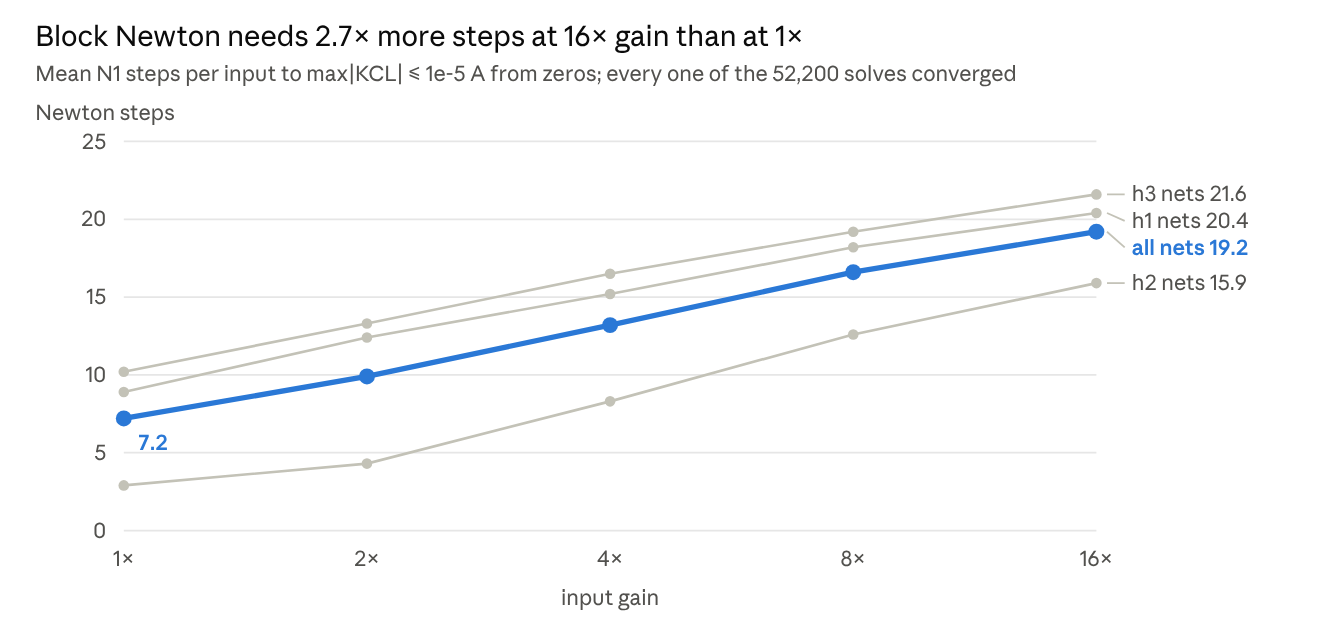
\includegraphics[width=0.88\linewidth]{figures/newton_review/newton_steps_vs_gain.png}
\caption[Block Newton needs 2.7\ensuremath{\times} more steps at 16\ensuremath{\times} gain than at 1\ensuremath{\times}]{Block Newton needs 2.7\ensuremath{\times} more steps at 16\ensuremath{\times} gain than at 1\ensuremath{\times}. \emph{Source: exp-017 accuracy table
(\nolinkurl{reviews/figures/exp017/tables/accuracy.csv}), arm N1, current\_1e-05 stop;
29 networks \ensuremath{\times} 360 inputs per gain; per-network means averaged.}}
\label{fig:newton-review-newton-steps-vs-gain}
\end{figure}

\begin{itemize}
\item \textbf{Steps track the overshoot.} From zeros, the first full step lands near the
diode-free linear solution, which overshoots $V_{\mathrm{off}}$ by many $V_T$ at high
gain. Armijo then backtracks, and Newton walks down the exponential. Gain scales the
overshoot, so it scales the steps (worst case 17 at 1\ensuremath{\times}, 30 at
16\ensuremath{\times}). This explanation is cd-newton-gain H-001 and is not yet tested
formally.
\item \textbf{h2 nets are near-linear at 1\ensuremath{\times}.} They need 2.9 steps at
1\ensuremath{\times} because several trained h2 checkpoints barely turn their diodes on.
\item \textbf{No junction limiting is the main weakness.} Starting from the linear solution at
8\ensuremath{\times} makes Newton 2.5--5\ensuremath{\times} slower, and it overflows on
h1 nets and single h3w512 (\nolinkurl{tolerance_start_20261022}). CD from the same start
is unaffected (\ensuremath{\pm}5\%). The planned \nolinkurl{pnjlim} variant targets
exactly this.
\item \textbf{Newton held where CD failed.} Before the exp\_clip fix, dense-LU Newton passed
360/360 on MNIST h1 at gain 60, while the benchmark-profile CD passed the 10
\ensuremath{\mu}A audit on only 62--93/360 (exp-006).
\item \textbf{FP32 sets a floor, not the algorithm.} In FP32 the independent long-double KCL
audit passes 351/360 at $10^{-5}$ A on h1w128.
\end{itemize}

\subsection*{Performance}

Block Cholesky is the decisive implementation choice: it makes Newton
4.6\ensuremath{\times} faster than dense LU end to end, with no change in steps. Even
so, adaptive CD overtakes it from about 4\ensuremath{\times} gain.

\begin{figure}[htbp]
\centering
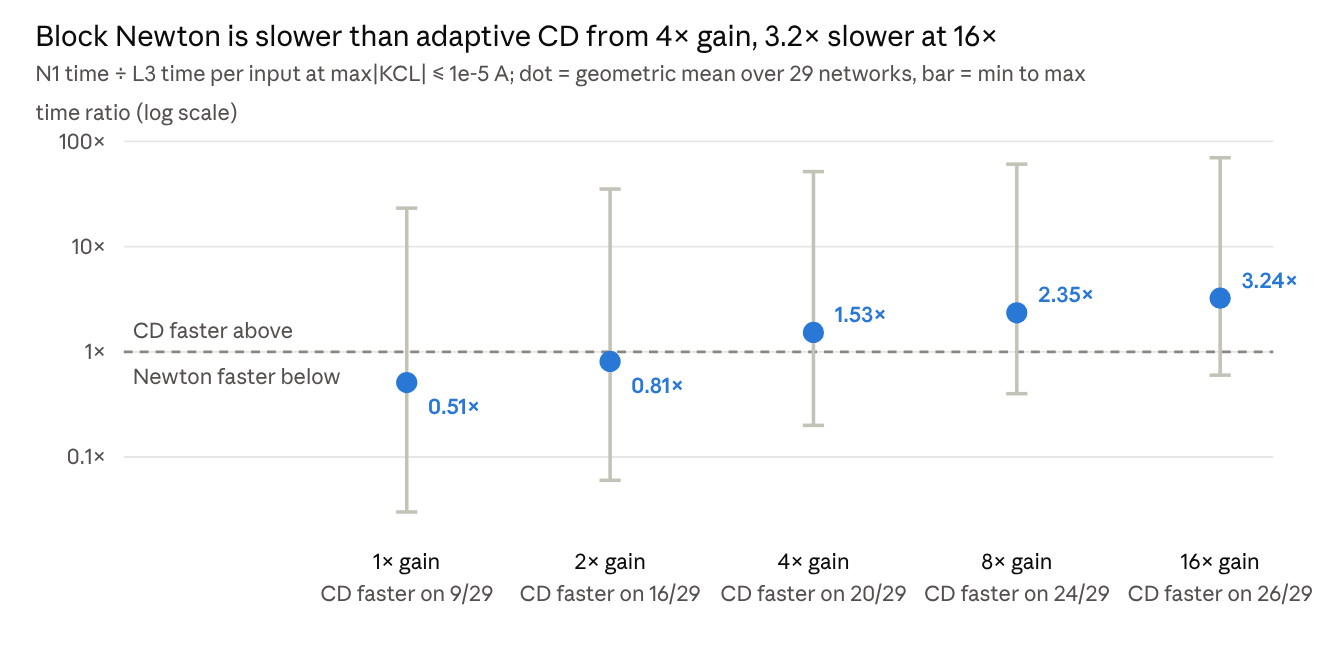
\includegraphics[width=0.88\linewidth]{figures/newton_review/n1_over_l3_by_gain.png}
\caption[Block Newton is slower than adaptive CD from 4\ensuremath{\times} gain, 3.2\ensuremath{\times} slower at 16\ensuremath{\times}]{Block Newton is slower than adaptive CD from 4\ensuremath{\times} gain, 3.2\ensuremath{\times} slower at 16\ensuremath{\times}. \emph{Source: exp-017 timing table
(\nolinkurl{reviews/figures/exp017/tables/timing.csv}), current\_1e-05 stop, local i9
core 0, 60 timing inputs (\nolinkurl{np.linspace(0, 359, 60)}); L3 time includes a
per-sweep residual check worth 1.3--1.9\ensuremath{\times}.}}
\label{fig:newton-review-n1-over-l3-by-gain}
\end{figure}

\textbf{Newton against Newton}

\begin{itemize}
\item \textbf{Dense LU \ensuremath{\to} block Cholesky:} the steps are the same, and the
speedup is 2.0--104\ensuremath{\times}, geometric mean 4.6\ensuremath{\times}
(\nolinkurl{established_gain_20261022}, 22 checkpoints, 360 inputs). The largest gains
are on h1 nets, where the block solve never factors the hidden layer.
\item \textbf{Of that saving, symmetry alone is worth 1.9--2.1\ensuremath{\times}.} A dense
Cholesky of $S$ already gets it. The layer structure adds 3--230\ensuremath{\times} on
h1 nets but only 1.2--1.5\ensuremath{\times} on h2/h3, where a general $2w^3$ Schur
product dominates.
\item \textbf{Cost per step} (fitted on exp-017): with $L$ free layers,
$N_w$ weights, $d$ hidden layers and hidden width $w$,
\[
\begin{aligned}
t_{\mathrm{Newton}}
&=0.11\,\mathrm{ms}\,L+1.4\,\mathrm{ns}\,N_w\\
&\quad+76\,\mathrm{ps}\,(d-1)w^3
+168\,\mathrm{ps}\,\max(d-2,0)w^3.
\end{aligned}
\]
A CD sweep costs $0.18\,\mathrm{ms}\,L+0.75\,\mathrm{ns}\,N_w$,
with no $w^3$ term.
\end{itemize}

\textbf{Newton against CD and SPICE}

\begin{itemize}
\item \textbf{Against framework CD (L3),} N1 is faster at 1--2\ensuremath{\times} gain and
slower from 4\ensuremath{\times}. At $10^{-9}$ A the crossover moves up to about
4\ensuremath{\times} (geometric mean 1.09\ensuremath{\times}), because Newton's
quadratic tail is cheap.
\item \textbf{Against LITE} (the same CD iterates without framework overhead), N1 loses on
139/145 pairs at $10^{-5}$ A, with a geometric mean of 8.3\ensuremath{\times}. It wins
only where it needs about one step (near-linear nets at 1--2\ensuremath{\times}). N1
itself has not been leaned out (NumPy per-step overhead), so small-net margins are upper
bounds.
\item \textbf{Hybrid:} CD to $10^{-2}$ A, then 1--2 block-Newton steps, is
1.15--2.1\ensuremath{\times} faster than CD alone at $10^{-9}$ A. At $10^{-5}$ A one
block step on $w=1024$ (about 57 ms) costs as much as about 20 sweeps, so the hybrid
pays only at tight tolerances.
\item \textbf{Against ELDO,} local Newton is 80--4,100\ensuremath{\times} faster per input
than the paper's interactive ELDO loop. Most of that is ELDO's per-analysis setup: batch
\nolinkurl{.DC DATA} is 12--33\ensuremath{\times} cheaper per input. The remaining
11--53\ensuremath{\times} is formulation (MNA has about 2.9\ensuremath{\times} the
unknowns) times iterations.
\end{itemize}

\subsection*{Side by side}

Block-Cholesky Newton (N1) is the solver to cite, with dense LU as the baseline. The
planned extensions are listed for context.

\begin{description}[style=nextline]
\item[Block Cholesky (N1)]
\textbf{Code:} \nolinkurl{solver.py}, \nolinkurl{backend='block_cholesky'}.
\textbf{Linear work per step:} Schur product + Cholesky per layer after the first;
$O(wm^2)$ on h1. \textbf{Step rule:} Armijo. \textbf{Steps vs N1:} same. \textbf{Where
it is used:} exp-017, established\_gain. \textbf{Verdict:} Default; the fair Newton for
R1.3.
\item[Dense LU]
\textbf{Code:} \nolinkurl{solver.py}, \nolinkurl{backend='dense_lu'}. \textbf{Linear
work per step:} $\frac{2}{3}n^3$ general LU of the full $J$. \textbf{Step rule:} Armijo.
\textbf{Steps vs N1:} same. \textbf{Where it is used:} exp-001, exp-006 (MNIST),
established\_gain. \textbf{Verdict:} Baseline only; 4.6\ensuremath{\times} slower than
N1.
\item[Junction-limited]
\textbf{Code:} none (cd-newton-gain H-004). \textbf{Linear work per step:} as N1.
\textbf{Step rule:} \nolinkurl{pnjlim} + Armijo. \textbf{Steps vs N1:} ---.
\textbf{Where it is used:} planned. \textbf{Verdict:} Not implemented.
\item[Newton--Krylov]
\textbf{Code:} none (cd-newton-eldo H-005). \textbf{Linear work per step:} PCG,
linear-network preconditioner. \textbf{Step rule:} Armijo. \textbf{Steps vs N1:} ---.
\textbf{Where it is used:} planned (exp-012). \textbf{Verdict:} Not implemented.
\end{description}

\subsection*{Open issues and next steps}

The biggest gap is that our Newton has no junction limiting. A reviewer can fairly say
that SPICE-grade Newton would take fewer steps at high gain.

\begin{itemize}
\item[$\square$] \textbf{Implement junction-limited Newton (H-004).} Add \nolinkurl{pnjlim} on
$|v|-V_{\mathrm{off}}$ to N1 and rerun the high-gain pairs. It also makes the
linear-solution start usable, which currently overflows.
\item[$\square$] \textbf{Lean out N1 before quoting LITE margins on small nets.} Remove the NumPy
per-step overhead and the \nolinkurl{np.diag} and temporary allocations (about 17\% of
h2w1024). Form the symmetric Schur product with a syrk (about half its flops).
\item[$\square$] \textbf{Run Newton--Krylov (H-005, exp-012).} It is the clean test of whether CD's
advantage is just "no factorization".
\item[$\square$] \textbf{Re-time at 360 inputs if these numbers enter the paper.} exp-017 local timing
used 60 inputs (\nolinkurl{np.linspace(0, 359, 60)}); accuracy and step counts used all
360.
\item[$\square$] \textbf{Settle the stop rule (cd-newton-gain H-005).} Compare the Jacobian-scaled
residual with the voltage-change stop across gains and methods.
\end{itemize}

% END NEWTON SOLVER REVIEW

\clearpage

\section*{H1. Much of the speed-up came from how ELDO was run}

\decision{Should I rerun the simulations in batch mode?}

\claim{Two choices in how the paper ran ELDO, neither related to coordinate
descent, made ELDO much slower than it needs to be. (a) Each input was
applied as its own interactive analysis (\texttt{eldo -inter}, then
\texttt{SET P} and \texttt{RUN} per input). A single batch analysis over
all inputs (\texttt{.DATA} plus \texttt{.DC DATA=}) gives identical
solutions at a fraction of the cost. (b) Every resistor value was written
as a global \texttt{.PARAM}, which makes ELDO slow to load the netlist.
With the values written inline, loading takes seconds, and the largest
networks, which the paper could not simulate, can be simulated.}

\subsection*{(a) Batch sweep instead of interactive mode}

\evidence
% campaigns/cd-newton-eldo/series/001-eldo-gap/results/exp-016.md
% solvers/eldo_batch_dc_20261023/summary.json
The paper's own netlists, double Shockley, 20 inputs per network, on
maxicao. Time per input once ELDO has started:

\begin{center}
\small
\begin{tabular}{lrrr}
\toprule
Network & Interactive (paper) & Batch & Factor \\
\midrule
h1w128 & 63 ms   & 7 ms   & 8.9$\times$ \\
h2w128 & 1.33 s  & 107 ms & 12.5$\times$ \\
h2w256 & 10.06 s & 307 ms & 32.8$\times$ \\
\bottomrule
\end{tabular}
\end{center}

\begin{itemize}
\item Every \texttt{RUN} starts a new DC analysis, and the first
point of each analysis costs 1.1~s (h2w128) and 9.8~s (h2w256) of ELDO
CPU, whatever the number of Newton iterations and even when no parameter
changed. Later points of a batch sweep cost 103 and 262~ms. ELDO's
profile attributes the first-point cost to rebuilding the sparse matrix
structure (about 60\%) and to a routine that appears to select pivots
(16--28\%). The
fill-in ELDO reports changes from input to input in interactive mode and
stays fixed through a batch sweep.
% campaigns/pilots/eldo-reorder-probe.md; solvers/eldo_reorder_20261024
% campaigns/cd-newton-eldo/series/002-cd-newton-regimes/experiments/exp-017-maxicao-paper-matrix.md
\end{itemize}

\subsection*{(b) Resistor values written inline}

\evidence
% exp-016 (.PARAM netlists, batch launch with one input); exp-017 (inline)
ELDO start-up CPU (loading and set-up, before the DC solve), same networks:

\begin{center}
\small
\begin{tabular}{lrr}
\toprule
Network & \texttt{.PARAM} netlist & Values inline \\
\midrule
h1w128 & 4.8 s & 0.8 s \\
h2w128 & 15 s  & 1.0 s \\
h2w256 & 196 s & 2.1 s \\
\bottomrule
\end{tabular}
\end{center}

\begin{itemize}
\item The netlists could not be simulated because the resistors were the .PARAM values. If the resistor values are written directly in the netlist, the netlist generation is much faster
\item With the values inline, ELDO simulated all four networks the
paper reported as infeasible (double and single Shockley, h2w1024 and
h3w512).
\end{itemize}

\begin{itemize}
\item \emph{Training.} In training every SGD update changes the
conductances, so ELDO must stay in an interactive session (a relaunch
pays the start-up again).
\end{itemize}

% -------------------------------------------------------------------
\section*{H2. Many of the networks simulated in the paper were near-linear}

\decision{Do I retrain the linear or near-linear networks, or do I increase the input gain?}

\claim{At the trained input gain, 9 of the 28 single- and double-Shockley
networks are linear to working precision: block Newton started from zero
converges in one step (max$|\mathrm{KCL}| \le 10^{-5}$~A), and ELDO in 3
iterations, its minimum. They include the four networks with the largest
published speed-ups, h2w256 and h2w512 of both families
(175--1756$\times$). }

\evidence
% campaigns/cd-newton-eldo/series/002-cd-newton-regimes/experiments/exp-017-maxicao-paper-matrix.md
% figures/exp017/tables/{accuracy,eldo}.csv (gain 1; N1 rows; E1 rows)
Paper networks at the trained gain, on maxicao (exp-017). Newton is block
Cholesky started from zero, over all 360 validation inputs. ELDO is the
batch sweep at its default tolerances, over 60 of them. $\dagger$ marks the
near-linear networks.

\begin{center}
\small
\begin{tabular}{llrrrr}
\toprule
Family & Network & Published & \multicolumn{2}{c}{Newton steps, mean (max)} & ELDO iterations \\
\cmidrule(lr){4-5}
 & & speed-up & to $10^{-5}$~A & to $10^{-9}$~A & per input \\
\midrule
Single & h1w64            & 8.2  & 5.8 (10)  & 6.5 (10)  & 7.6 \\
       & h1w128           & 4.0  & 12.4 (14) & 13.3 (15) & 10.1 \\
       & h1w256           & 11.8 & 11.6 (13) & 12.6 (14) & 11.7 \\
       & h1w512           & 33.0 & 10.8 (13) & 11.7 (14) & 12.3 \\
       & h1w1024          & 132  & 11.4 (13) & 12.3 (14) & 13.6 \\
       & h2w64            & 4.3  & 7.7 (11)  & 8.4 (12)  & 8.3 \\
       & h2w128           & 27.3 & 7.2 (10)  & 8.0 (11)  & 9.7 \\
       & h2w256 $\dagger$ & 175  & 1.0 (1)   & 1.7 (2)   & 3.0 \\
       & h2w512 $\dagger$ & 1252 & 1.0 (1)   & 1.0 (2)   & 3.0 \\
       & h2w1024 $\dagger$& --   & 1.0 (1)   & 1.0 (2)   & 3.0 \\
       & h3w64            & 1.2  & 9.4 (14)  & 10.2 (15) & 10.6 \\
       & h3w128           & 35.6 & 13.3 (17) & 14.2 (17) & 12.5 \\
       & h3w256           & 98.2 & 10.9 (15) & 11.6 (16) & 11.7 \\
       & h3w512           & --   & 13.5 (16) & 14.1 (17) & 12.2 \\
\addlinespace
Double & h1w64            & 3.7  & 8.6 (12)  & 9.4 (12)  & 9.4 \\
       & h1w128 $\dagger$ & 15.4 & 1.2 (3)   & 2.0 (3)   & 3.1 \\
       & h1w256           & 16.9 & 9.0 (11)  & 9.9 (12)  & 10.9 \\
       & h1w512           & 39.6 & 9.0 (11)  & 10.0 (12) & 11.6 \\
       & h1w1024          & 133  & 9.1 (11)  & 10.0 (12) & 12.4 \\
       & h2w64 $\dagger$  & 4.7  & 1.0 (1)   & 2.0 (2)   & 3.0 \\
       & h2w128           & 37.4 & 7.5 (9)   & 8.4 (10)  & 9.2 \\
       & h2w256 $\dagger$ & 257  & 1.0 (1)   & 1.9 (2)   & 3.0 \\
       & h2w512 $\dagger$ & 1756 & 1.0 (1)   & 1.1 (2)   & 3.0 \\
       & h2w1024 $\dagger$& --   & 1.0 (1)   & 1.0 (2)   & 3.0 \\
       & h3w64            & 5.0  & 12.9 (16) & 13.8 (17) & 13.9 \\
       & h3w128           & 54.0 & 9.9 (14)  & 10.7 (14) & 9.9 \\
       & h3w256           & 303  & 7.2 (10)  & 8.0 (11)  & 8.4 \\
       & h3w512 $\dagger$ & --   & 1.0 (1)   & 2.0 (2)   & 3.0 \\
\bottomrule
\end{tabular}
\end{center}

\begin{itemize}
\item The other 19 networks need 6--14 Newton steps on average, at most 17.
ELDO's iteration counts track our Newton's closely there (8--14 per
input).
\item At the trained gain ELDO's counts are complete: it needed G ramping
(a continuation method whose work its iteration count leaves out) on only
one input of the 60, on one network (double h3w64).
\end{itemize}

% -------------------------------------------------------------------
\section*{H3. The published CD implementation was far from optimal}

\decision{Should I use the improved CD version?}

\claim{The published CD times understate what CD can do, for two separate
reasons. (1) The implementation spent its time waiting on the framework,
not on arithmetic. (2) The over-relaxation factor was fixed, where it can
be adapted to the operating point.}

\subsection*{(1) Implementation}

\evidence
% solvers/cd_fix_20261023/README.md (profiling); commits 7a4c845,
% 393248c, cd7a472, 9ff6ff7, 57a38fb on branch cd-solver-fixes
\begin{itemize}
\item \emph{Many small operations.} Profiled at batch 1 on CPU (local
workstation), the matrix--vector products are only 2--20\% of a sweep. Each
hidden-layer update issued about 100 small PyTorch operations at
4--6~$\mu$s each, whatever their size. Decisions taken on the host inside
every update (\texttt{any()} checks, masked indexing, early exits,
finiteness checks) made the host wait for each result before continuing.
There was also avoidable work: a coefficient was recomputed from the full
weight matrices on every update, and the single-diode update solved both
diode orientations for every node and discarded one.
\item \emph{Lambert $W$, correctness.} The exponent of the Lambert-$W$
argument was clipped at \texttt{exp\_clip}. Above about 3--8$\times$ the
trained input gain the clipped argument gave far too large a voltage, and
CD stopped at a false fixed point with errors of tens of volts. Computing
$\log z$ directly and evaluating the asymptotic series from it removes the
clipping (commit 393248c). At the trained gain the results are unchanged,
so the paper's numbers are not affected.
\item \emph{Lambert $W$, speed and precision.} The library used for $W$
(\texttt{torchlambertw}) computes in FP32, stops at an absolute $10^{-6}$,
and loops in Python until every element has converged. We replaced it with
Halley's method in the working precision: at most 4 steps over the whole
FP64 range, agreement with SciPy to $4\times10^{-16}$, and no decision on
the host.
\item \emph{Fix.} With $W$ computed this way, the whole coordinate update
can be written without host decisions, fused, and compiled with
\texttt{torch.compile}. It performs the same iterations as the repaired
CD (sweep counts within 0.03 on every paper network and gain) at a lower
cost per sweep: median 1.7~ms $\to$ 0.79~ms at the trained gain.
\end{itemize}

\subsection*{(2) Over-relaxation}

\begin{itemize}
\item Linearised at equilibrium, this CD is SOR on a consistently ordered
(2-cyclic) Jacobian, so Young's theory predicts its convergence rate. The
optimal $\omega$ falls as the diodes conduct, so the paper's fixed
$\omega$ (1.0, 1.2 or 1.4 per network) is wrong at most gains.
\item Estimating $\omega$ from the last sweeps cuts the number of sweeps
(table below). It is slower on a few networks at low gain, at worst
0.83$\times$ the fixed-$\omega$ speed.
\end{itemize}

\subsection*{Gains}

% figures/exp017/tables/timing.csv; solvers/maxicao_matrix_20261024/ratios.py
All 28 paper networks, maxicao, one core, one input at a time; time per
input at max$|\mathrm{KCL}| \le 10^{-5}$~A, relative to the repaired CD
(geometric mean over networks; exp-017):

\begin{center}
\small
\begin{tabular}{lrrrrr}
\toprule
Input gain & 1$\times$ & 2$\times$ & 4$\times$ & 8$\times$ & 16$\times$ \\
\midrule
Fused (1)                         & 2.19$\times$ & 2.29$\times$ & 2.41$\times$ & 2.43$\times$ & 2.46$\times$ \\
Fused + adaptive $\omega$ (1)+(2) & 2.69$\times$ & 3.07$\times$ & 3.51$\times$ & 3.69$\times$ & 4.04$\times$ \\
\addlinespace
Sweeps, adaptive / fixed $\omega$ & 0.77 & 0.71 & 0.66 & 0.63 & 0.58 \\
\bottomrule
\end{tabular}
\end{center}

\begin{itemize}
\item Fused CD with adaptive $\omega$ is faster than the repaired CD on all
28 networks at every gain, by 1.5--8.8$\times$. At the paper's stop
(relative voltage change $10^{-5}$) the two speed-up rows become
2.7--3.1$\times$ and 3.0--4.0$\times$.
\item Against the published CD times, fused CD with adaptive $\omega$ is
3.6--17$\times$ faster at the trained gain (geometric mean 5.6$\times$
double, 7.8$\times$ single). The published times include Python start-up
and model loading for the whole 360-input run, so this overstates the
implementation gain, most on the small networks.
% Provenance of the published CD times: data/timing/figure_inputs/*/
% combined_latest_by_hidden.csv, column coord_user_time_seconds (process
% user CPU of the validation run). The maxicao paper-run log for double
% h2w256 shows 7.3 s against 16.8 s in the table; the run behind the table
% is not yet located.
\end{itemize}

\objections
\begin{itemize}
\item \emph{Is Newton equally optimised?} Newton's cost is the
block-Cholesky factorisations and solves, which run in optimised LAPACK
routines called from SciPy (OpenBLAS, one thread, the same as CD); only
the loop over Newton steps and layer blocks is Python.
\end{itemize}

% -------------------------------------------------------------------
\section*{H4. When CD beats Newton}

% TODO (moved out of H2 on 2026-10-25, to be written here): the gain sweep
% from exp-017. From 1x to 16x, median Newton steps 8 -> 20 and CD sweeps
% (fused, adaptive omega) 17 -> 12; ELDO needed G ramping on 1/1/4/14/19 of
% 28 networks (recount from completed runs only), DC CPU per input 0.43 s ->
% 5.2 s (geometric mean), up to 5,400 s (single h3w512, 16x); ELDO's
% iteration counts omit G-ramping work, so they are not comparable at high
% gain. Objections: realism of scaled inputs (mean accuracy 0.92 -> 0.85,
% worst network 0.83 -> 0.42); our Newton has no junction limiting.

\claim{For both methods, time to solve = iterations $\times$ cost per
iteration, and the two methods scale in opposite ways on both factors. The
more nonlinear the network, the better CD converges and the worse Newton
does. CD therefore wins once the network is nonlinear, and by more the
wider and deeper it is.}

\textbf{Cost per iteration} depends on the architecture
(Figure~\ref{fig:cost-per-iteration}).
\begin{itemize}
\item A CD sweep costs a fixed 0.18~ms per layer plus 0.75~ns per weight.
At these sizes the fixed part dominates: from $9\times10^3$ to
$1.2\times10^6$ weights a sweep only grows from 0.36 to 1.4~ms.
\item A block-Cholesky Newton step has the same two terms (0.11~ms per
layer, 1.4~ns per weight) plus a dense factorisation for every hidden
layer after the first, which grows with the cube of the width. With one
hidden layer there is none, and a step (0.2--0.4~ms) is cheaper than a
sweep.
\item With two or three hidden layers a Newton step costs more than a
sweep from width 128, and the dense part takes over: from width 256 to
1024 with two hidden layers, a step costs 3 to 53 sweeps (1.9 against
0.65~ms, 74 against 1.4~ms).
\end{itemize}

\begin{figure}[htbp]
\centering
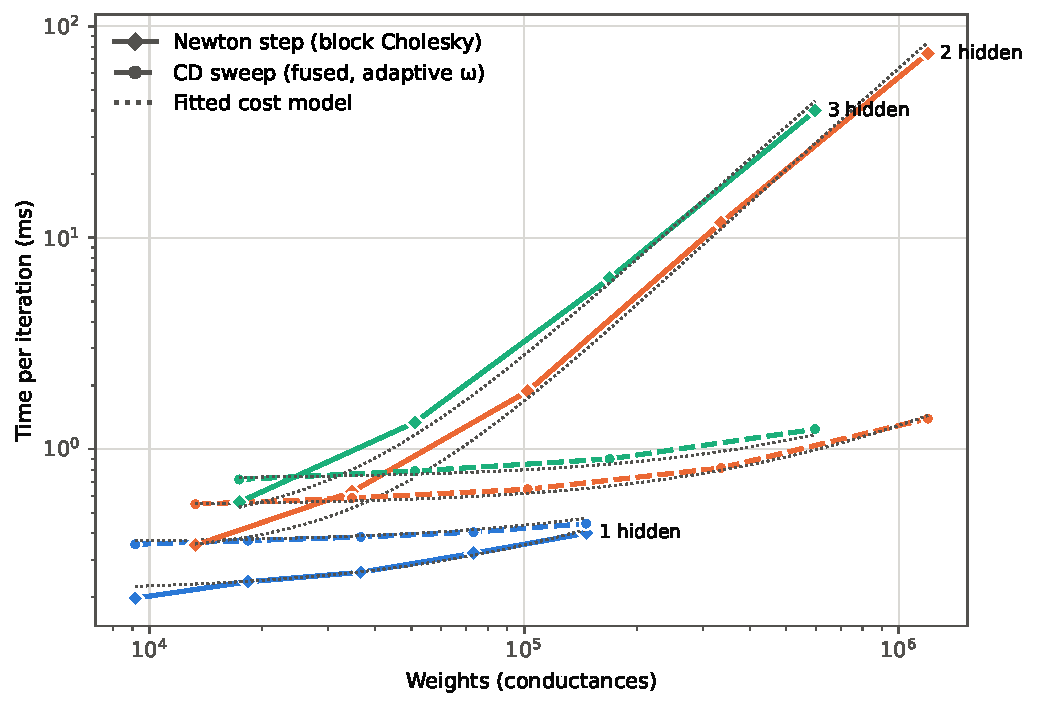
\includegraphics[width=0.75\textwidth]{h4_cost_per_iteration.pdf}
\caption[Time per iteration against the number of weights]{Time per
iteration against the number of weights, for $d = 1$, 2 and 3 hidden
layers of width $w$. Newton step: block Cholesky, at the
max$|\mathrm{KCL}| \le 10^{-6}$~A stop. CD sweep: fused CD with adaptive
$\omega$, at its own voltage-change stop (rtol $10^{-6}$); the
max$|\mathrm{KCL}|$ stops are timed sweep by sweep with a residual
evaluation after every sweep, which is not part of a sweep. Median over the
five gains and both diode families, 60 timing inputs, one core of maxicao.
Dotted: cost models fitted by least squares in relative error over the 14
architectures, with $L = d+1$ layers of nodes (hidden and output) and $N$
weights:
\[\begin{aligned}
t_\mathrm{CD} &= 0.18~\mathrm{ms}\cdot L + 0.75~\mathrm{ns}\cdot N,\\
t_\mathrm{Newton} &= 0.11~\mathrm{ms}\cdot L + 1.4~\mathrm{ns}\cdot N
  + 76~\mathrm{ps}\cdot(d-1)\,w^3 + 168~\mathrm{ps}\cdot\max(d-2,0)\,w^3.
\end{aligned}\]
The first two terms are fixed overhead per layer and work per weight (for
Newton, the residual and Jacobian evaluations, one per line-search trial).
The $w^3$ terms are Newton's dense linear algebra: for each of the $d-1$
hidden layers after the first, a Schur complement and its Cholesky factor
($2w^3 + w^3/3$ flops, about 31~GFLOP/s), and for each of the $d-2$ links
between those layers a triangular solve against $w$ right-hand sides
($2w^3$ flops, about 12~GFLOP/s). The CD model is within 6\% of every
point. The Newton model is within 16\%; it is low at width 128 and high at
the largest sizes, because BLAS throughput rises with the block size.}
\label{fig:cost-per-iteration}
\end{figure}
% figures/exp017/tables/timing.csv (arms N1 current_1e-06, L3 rtol_1e-06);
% solvers/maxicao_matrix_20261024/h4_figures.py prints the fit and per-point errors

\textbf{Iterations} depend on the nonlinearity
(Figure~\ref{fig:iterations}; per-network numbers in the appendix). The
gain drives the hidden diodes into their exponential region: their share
rises with the gain on every network except single h3w128, where it stays
at 62--66\%.
\begin{itemize}
\item Newton takes more steps as the gain rises, on every network: about
three more per doubling of the gain (median 3.1, range 1.9--3.8), from
1--14 at $1\times$ (one on the near-linear networks of H2) to 13--26 at
$16\times$.
\item Along each network, more nonlinear diodes means more Newton steps,
but the share does not set the count across networks: single h1w512 and
h1w1024 need 11 steps with 8--10\% of the diodes nonlinear, and single
h3w128 goes from 14 to 22 steps while its share stays flat. The step count
follows the gain more closely than the share.
\item CD needs fewer sweeps as the gain rises, on 27 of the 28 networks
(single h3w128 goes from 12 to 13). It needs more on deeper networks: the
median goes from 8 to 6 sweeps with one hidden layer, from 23 to 15 with
two and from 24 to 15 with three, between $1\times$ and $16\times$.
\end{itemize}

\begin{figure}[htbp]
\centering
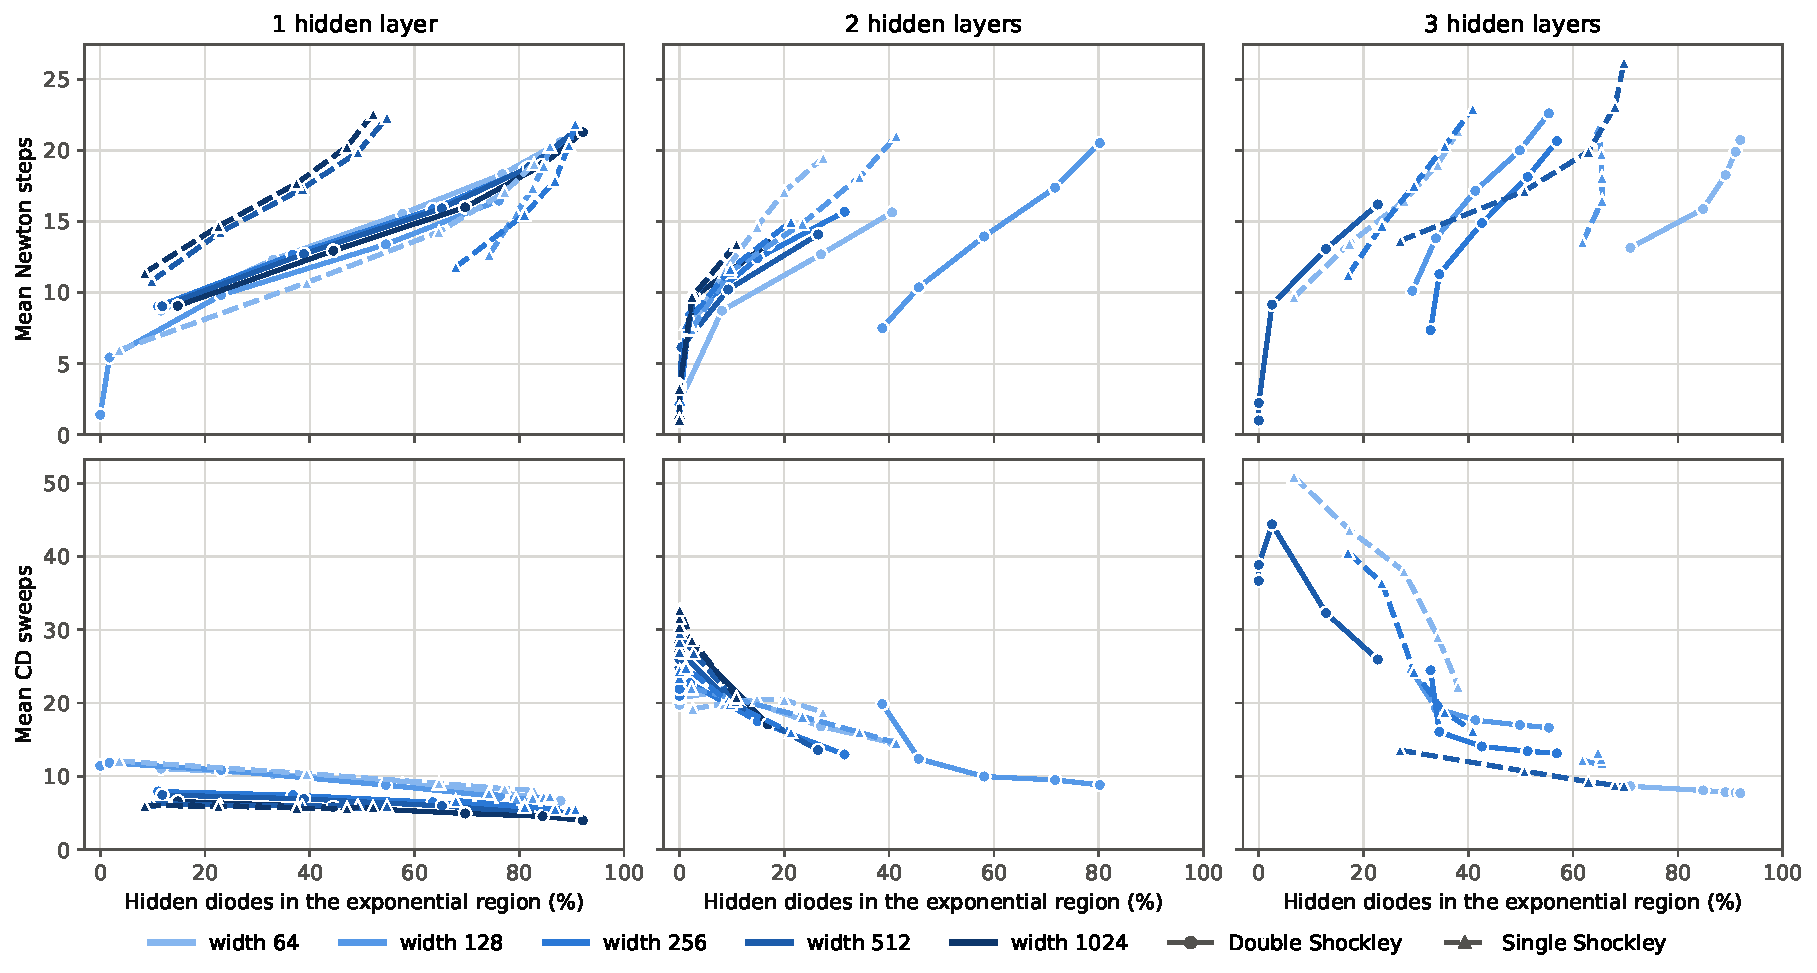
\includegraphics[width=\textwidth]{h4_iterations_vs_nonlinearity.pdf}
\caption[Iterations against the share of nonlinear diodes]{Mean Newton
steps (top, block Cholesky) and CD sweeps (bottom, fused with adaptive
$\omega$) to max$|\mathrm{KCL}| \le 10^{-6}$~A from zero, against the share
of hidden diodes in the exponential region; columns are 1, 2 and 3 hidden
layers. A diode counts as nonlinear when its incremental conductance is at
least 10\% of the node's resistive self-conductance ($g_d \ge 0.1\,G_{ii}$)
at the $10^{-10}$~A reference state; the exponential makes the split sharp,
and thresholds of 1\% and 100\% change the shares by a few points only.
Each line is one network through the gains $1$, 2, 4, 8 and $16\times$,
which raise the share. Colour is the width; solid lines with circles are
double-Shockley networks, dashed lines with triangles single-Shockley.
Iterations and shares over all 360 validation inputs.}
\label{fig:iterations}
\end{figure}
% figures/exp017/tables/accuracy.csv (stop current_1e-06, arms N1 and L3) and
% diode_regions.csv (share_01); solvers/maxicao_matrix_20261024/h4_figures.py

Together: with one hidden layer both methods pay about the same per
iteration, and the one needing fewer iterations wins, Newton at low gain
and CD at high gain. With two and three hidden layers a Newton step costs
several sweeps from width 256, and once the network is nonlinear enough
for Newton to need more than a handful of steps, CD wins
(Figure~\ref{fig:cd-newton-eldo}).

\begin{figure}[htbp]
\centering
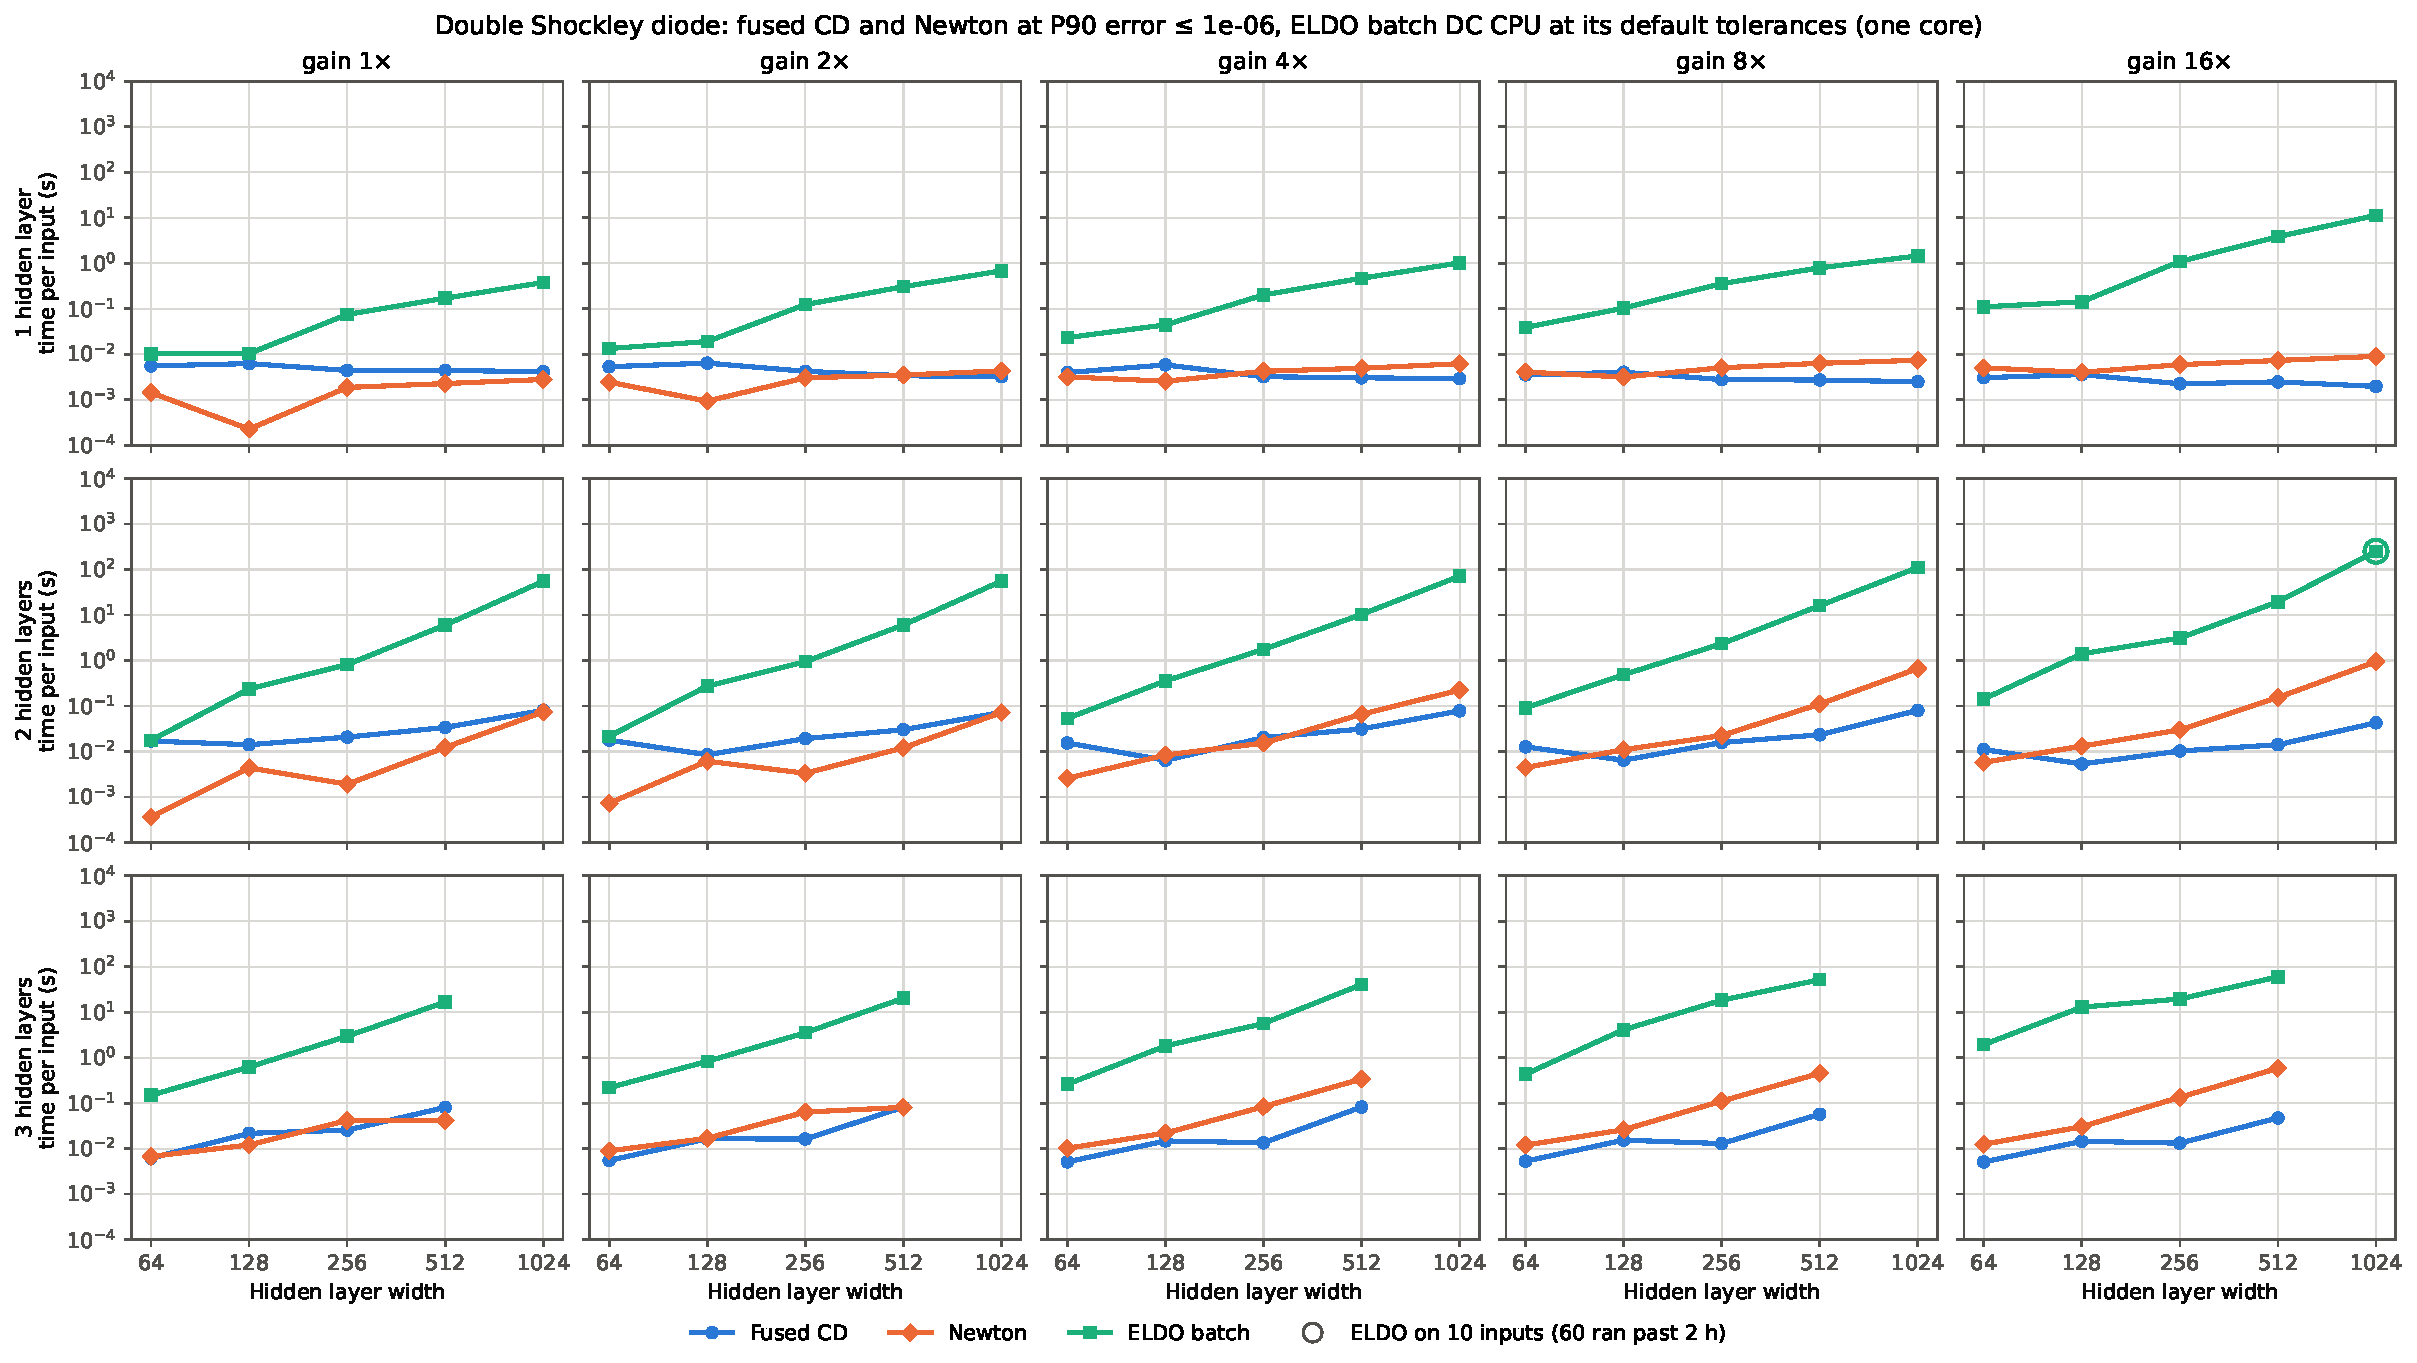
\includegraphics[width=\textwidth]{cd_newton_eldo_double.pdf}

\medskip

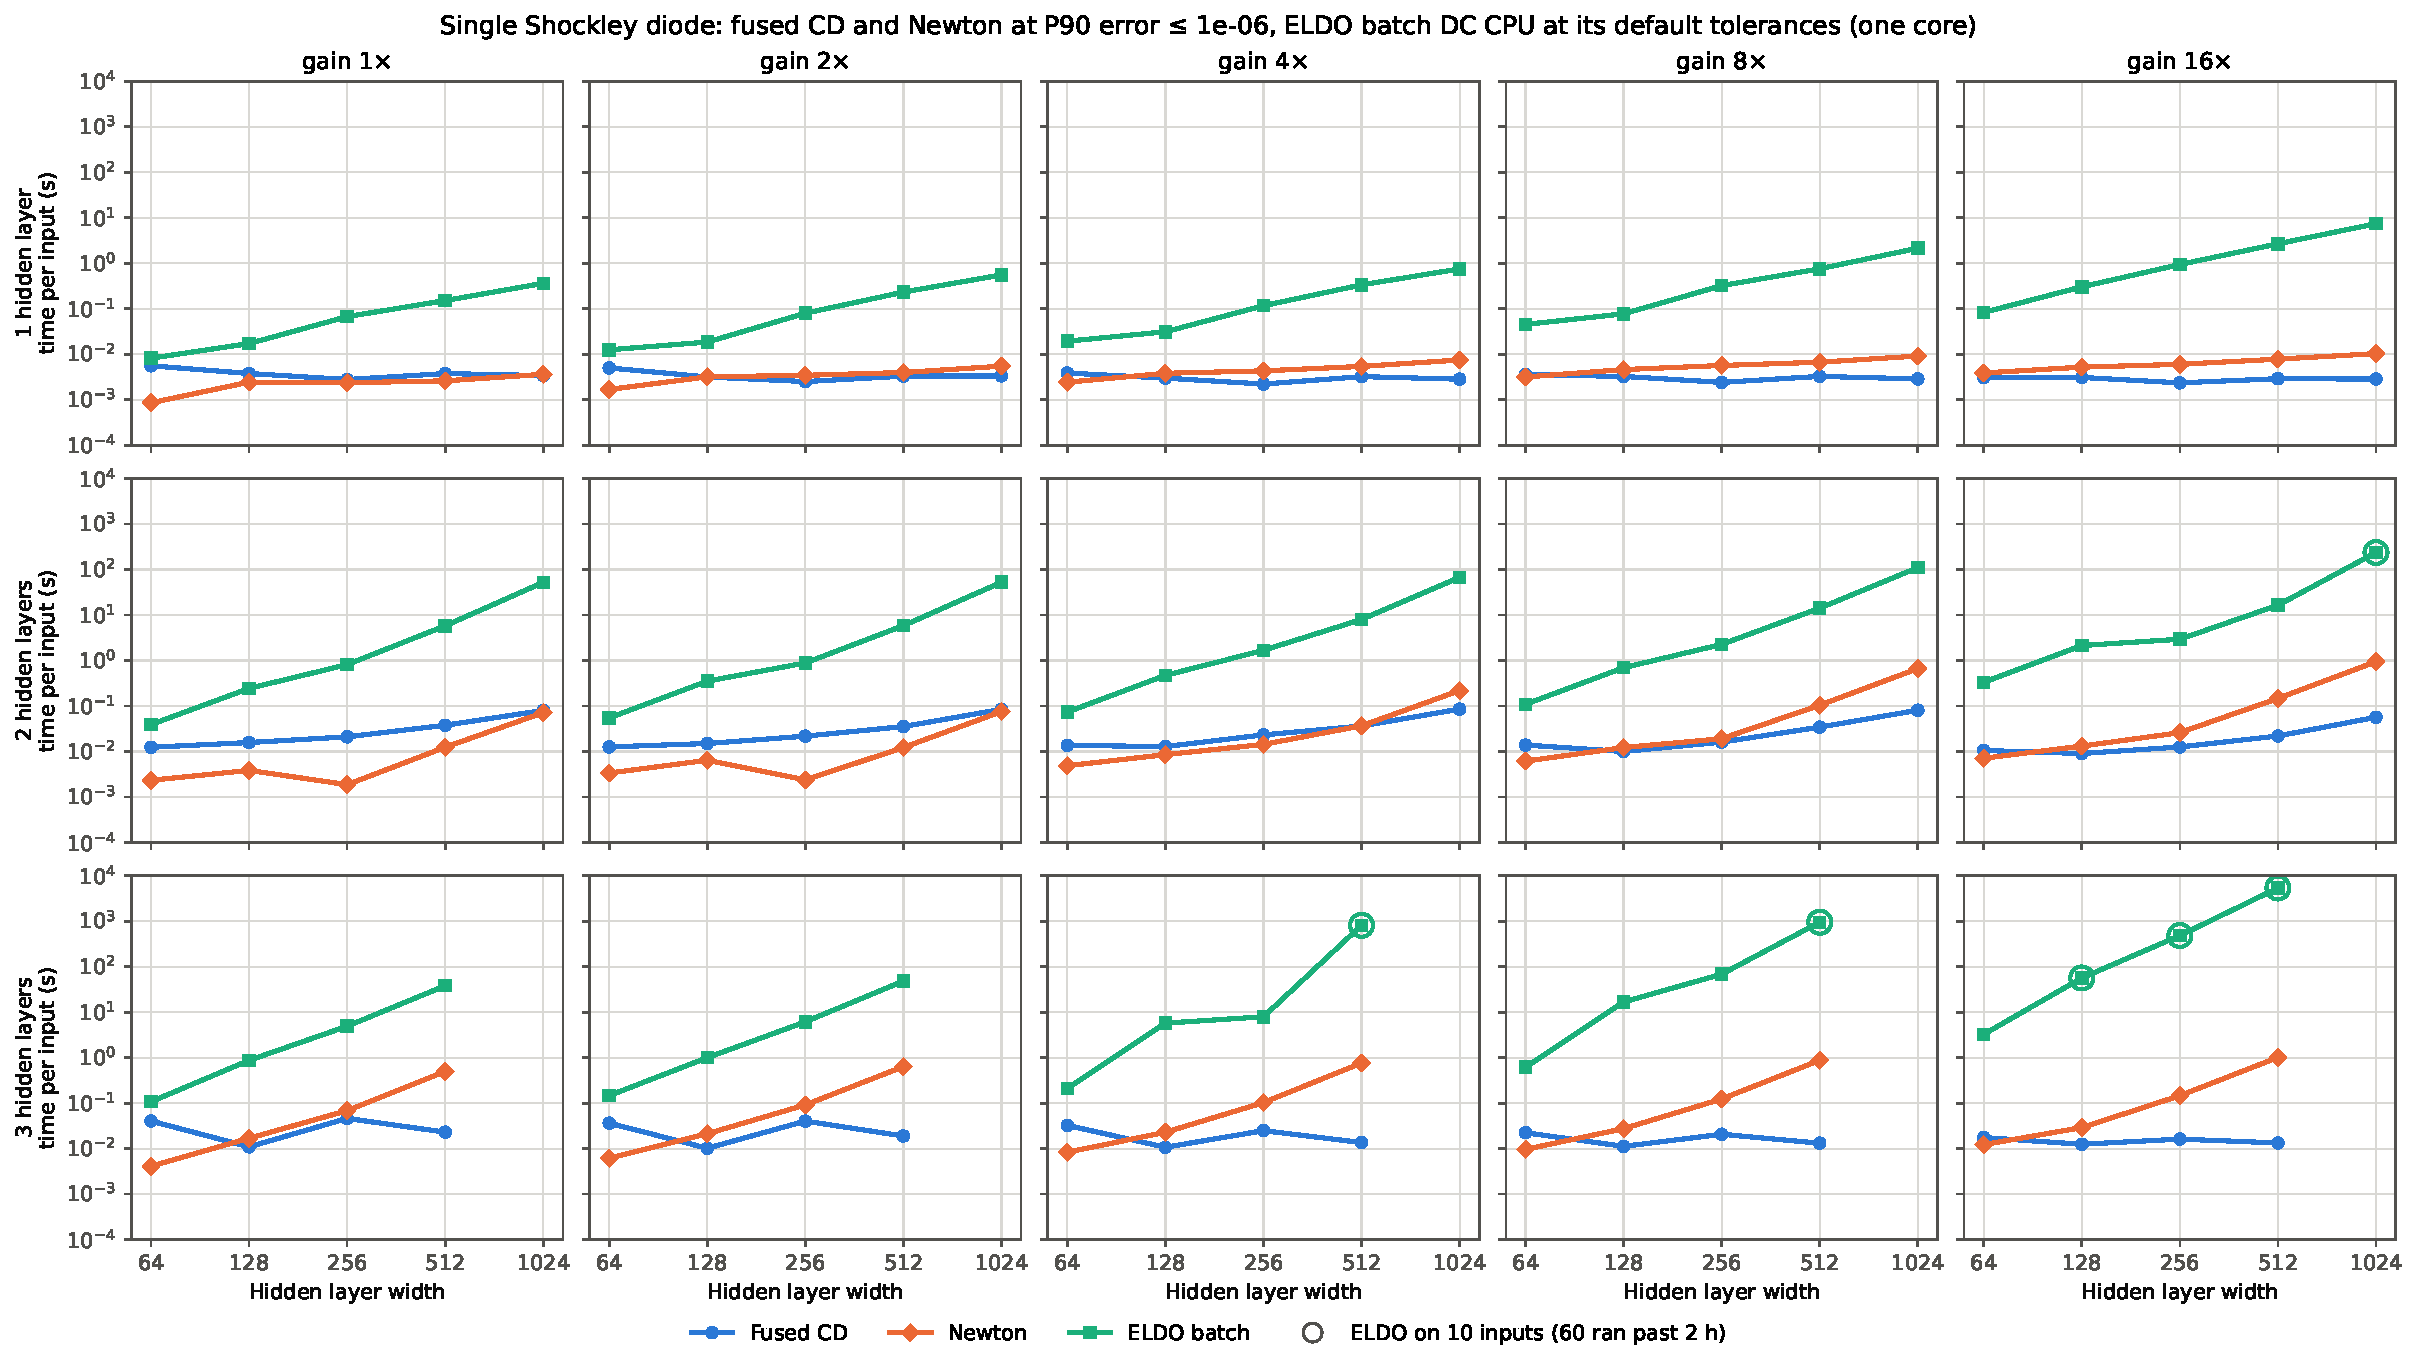
\includegraphics[width=\textwidth]{cd_newton_eldo_single.pdf}

\caption{Double-Shockley (top) and Single-Shockley (bottom) networks.
Time per input against hidden-layer width; rows are 1, 2 and 3 hidden
layers, columns the input gain. Fused CD (adaptive $\omega$) and Newton
are timed at matched accuracy (P90 relative error $\le 10^{-6}$ against
the $10^{-10}$~A reference); ELDO is batch DC CPU per input at its default
tolerances (about $10^{-5}$), without start-up. Circled ELDO points ran
on 10 inputs only. One core of maxicao.}
\label{fig:cd-newton-eldo}
\end{figure}

What the figures show:
\begin{itemize}
\item One hidden layer: CD and Newton both take 2--10~ms per input at all
widths. Newton is ahead at $1\times$, they are level by $4\times$, and CD
is slightly ahead from $8\times$.
\item Two hidden layers: at $1$--$2\times$ Newton wins up to width 512 and
the two are level at 1024, because Newton needs one step on these
near-linear networks (H2). From $4\times$ Newton's curve steepens (cubic
cost times more steps) and CD pulls away, by about $22\times$ on width
1024 at $16\times$.
\item Three hidden layers: on the double-Shockley networks CD and Newton
are level at $1$--$2\times$ and CD leads from $4\times$. On the
single-Shockley networks CD leads from width 128 at every gain: single
h3w512 is already nonlinear at the trained gain (14 Newton steps), where
CD is $22\times$ faster.
\item ELDO is 1--3 orders of magnitude slower than both everywhere, and
grows fastest with gain on three hidden layers (up to about 5000~s per
input on single h3w512 at $16\times$).
\item The CD times here are at the max$|\mathrm{KCL}|$ stops, which are
timed sweep by sweep with a residual evaluation after every sweep. That
makes a sweep 1.3--1.9$\times$ slower than at CD's own stop
(Figure~\ref{fig:cost-per-iteration}), while Newton computes the residual
anyway, so the CD margins are conservative.
\end{itemize}

% Synthetic PWL (exp-018, figures/exp018) removed on request: it is the double-Shockley
% law sampled at 200 points and repeats that result. Manuscript fix still needed:
% main2.tex says the PWL samples span [-2,2] V; the curve file spans [-3,3] V.
% TODO: the evidence, objections and needed lists below are from the
% earlier campaign and are still to be rewritten from exp-017.

\evidence
% campaigns/cd-newton-eldo/series/002-cd-newton-regimes/results/exp-004.md
% solvers/cd_fix_20261023/README.md (compiled + adaptive table)
\begin{itemize}
\item Published CD, trained gain: CD wins only on single h3w512
($2.6$--$4.8\times$). Block Newton wins on every h1 network and on
h2w256.
\item Published CD, $8\times$ gain: CD wins on h2w1024 ($2.5$--$9.4\times$)
and double h3w512 ($1.5$--$4.5\times$).
\item Optimised CD (compiled + adaptive $\omega$): at the trained gain CD
beats block Newton on double h2w1024, h3w256 and h3w512 and on single
h2w1024, h3w256 and h3w512. At $16\times$ the margin reaches $40\times$
(double h2w1024) and $90\times$ (single h3w512).
\item The margin shrinks as the tolerance tightens, because Newton
converges quadratically and CD linearly: on $8\times$ double h2w1024,
$9.4\times$ at $10^{-3}$~A down to $3.1\times$ at $10^{-9}$~A.
\item For reference against ELDO rather than Newton: on h2w1024 ELDO's
Newton fails and it falls back to conductance ramping, at about 1300~s per
input against 0.15~s for CD (R1.5 study).
\end{itemize}

\objections
\begin{itemize}
\item Same as H2 and H3: no junction limiting in our Newton, and the
crossover depends on the implementations.
\item ``Larger'' was tested only up to width 1024 with two to three hidden
layers on Digits. The wider MNIST networks are not yet usable: there the
benchmarked CD failed on most inputs (before the exponent fix), and only
dense-LU Newton was timed.
\item The reviewer also mentions ``related sparse solvers''. A
matrix-free Newton--Krylov (conjugate gradients with a linear-network
preconditioner) avoids factorisation, which is exactly CD's advantage here.
\end{itemize}


% -------------------------------------------------------------------

\section*{Draft reply}

\todo{Write once the decomposition table is filled. Proposed order: (1)
thank the reviewer and state the decomposition; (2) ELDO driving and the
netlist format (H1); (3) formulation (H5); (4) CD versus the best Newton,
with the regime map (H4, with H2 as the explanation); (5) implementation
(H3); (6) training (H6); (7) the local versus global Newton point; (8) the
changes to the manuscript.}

% -------------------------------------------------------------------
\section*{Appendix: H4 per network}

The numbers behind Figure~\ref{fig:iterations}.

\begin{center}
\small
\begin{tabular}{rr|ccccc}
\multicolumn{2}{c|}{Network} & \multicolumn{5}{c}{Newton steps / CD sweeps} \\
Hidden layers & Width & $1\times$ & $2\times$ & $4\times$ & $8\times$ & $16\times$ \\
\hline
\multicolumn{7}{l}{\emph{Double Shockley}} \\
1 & 64 & 9 / 11 & 12 / 10 & 16 / 9 & 18 / 8 & 21 / 7 \\
1 & 128 & 1 / 11 & 5 / 12 & 10 / 11 & 13 / 9 & 16 / 7 \\
1 & 256 & 9 / 8 & 13 / 7 & 16 / 6 & 19 / 6 & 21 / 5 \\
1 & 512 & 9 / 7 & 13 / 7 & 16 / 6 & 19 / 5 & 21 / 5 \\
1 & 1024 & 9 / 7 & 13 / 6 & 16 / 5 & 19 / 5 & 21 / 4 \\
\cline{1-7}
2 & 64 & 1 / 20 & 2 / 21 & 9 / 22 & 13 / 17 & 16 / 15 \\
2 & 128 & 7 / 20 & 10 / 12 & 14 / 10 & 17 / 10 & 21 / 9 \\
2 & 256 & 1 / 21 & 2 / 22 & 8 / 23 & 12 / 18 & 16 / 13 \\
2 & 512 & 1 / 25 & 2 / 26 & 6 / 27 & 10 / 20 & 14 / 14 \\
2 & 1024 & 1 / 27 & 1 / 28 & 3 / 30 & 10 / 27 & 13 / 17 \\
\cline{1-7}
3 & 64 & 13 / 9 & 16 / 8 & 18 / 8 & 20 / 8 & 21 / 8 \\
3 & 128 & 10 / 24 & 14 / 19 & 17 / 18 & 20 / 17 & 23 / 17 \\
3 & 256 & 7 / 24 & 11 / 16 & 15 / 14 & 18 / 13 & 21 / 13 \\
3 & 512 & 1 / 37 & 2 / 39 & 9 / 44 & 13 / 32 & 16 / 26 \\
\hline
\multicolumn{7}{l}{\emph{Single Shockley}} \\
1 & 64 & 6 / 12 & 11 / 10 & 14 / 9 & 17 / 8 & 19 / 8 \\
1 & 128 & 13 / 8 & 16 / 7 & 17 / 7 & 19 / 7 & 20 / 7 \\
1 & 256 & 12 / 7 & 15 / 6 & 18 / 6 & 20 / 5 & 22 / 6 \\
1 & 512 & 11 / 6 & 14 / 6 & 17 / 6 & 20 / 6 & 22 / 6 \\
1 & 1024 & 11 / 6 & 15 / 6 & 18 / 6 & 20 / 6 & 23 / 6 \\
\cline{1-7}
2 & 64 & 8 / 19 & 11 / 20 & 15 / 20 & 17 / 20 & 19 / 19 \\
2 & 128 & 7 / 22 & 11 / 21 & 15 / 18 & 18 / 16 & 21 / 15 \\
2 & 256 & 1 / 24 & 2 / 24 & 8 / 25 & 12 / 20 & 15 / 16 \\
2 & 512 & 1 / 27 & 1 / 28 & 4 / 30 & 10 / 27 & 13 / 20 \\
2 & 1024 & 1 / 30 & 1 / 32 & 3 / 33 & 10 / 29 & 13 / 21 \\
\cline{1-7}
3 & 64 & 10 / 51 & 13 / 44 & 16 / 38 & 19 / 29 & 21 / 22 \\
3 & 128 & 14 / 12 & 16 / 12 & 18 / 12 & 20 / 12 & 22 / 13 \\
3 & 256 & 11 / 41 & 15 / 36 & 18 / 24 & 20 / 19 & 23 / 16 \\
3 & 512 & 14 / 14 & 17 / 11 & 20 / 9 & 23 / 9 & 26 / 9 \\
\end{tabular}

\smallskip
Mean iterations to max$|\mathrm{KCL}| \le 10^{-6}$~A over all 360
validation inputs, for each diode family; Newton is
block Cholesky, CD the fused CD with adaptive $\omega$, both from zero.
\end{center}
% figures/exp017/tables/accuracy.csv, stop current_1e-06, arms N1 and L3

\begin{center}
\small
\begin{tabular}{rr|ccccc}
\multicolumn{2}{c|}{Network} & \multicolumn{5}{c}{Nonlinear diodes (\%)} \\
Hidden layers & Width & $1\times$ & $2\times$ & $4\times$ & $8\times$ & $16\times$ \\
\hline
\multicolumn{7}{l}{\emph{Double Shockley}} \\
1 & 64 & 12 & 33 & 58 & 77 & 88 \\
1 & 128 & 0 & 2 & 23 & 54 & 76 \\
1 & 256 & 11 & 37 & 63 & 81 & 90 \\
1 & 512 & 12 & 39 & 65 & 82 & 91 \\
1 & 1024 & 15 & 44 & 70 & 84 & 92 \\
\cline{1-7}
2 & 64 & 0 & $<1$ & 8 & 27 & 41 \\
2 & 128 & 39 & 46 & 58 & 72 & 80 \\
2 & 256 & 0 & $<1$ & 2 & 15 & 32 \\
2 & 512 & 0 & 0 & $<1$ & 9 & 26 \\
2 & 1024 & 0 & 0 & $<1$ & 3 & 17 \\
\cline{1-7}
3 & 64 & 71 & 85 & 89 & 91 & 92 \\
3 & 128 & 29 & 34 & 41 & 50 & 55 \\
3 & 256 & 33 & 34 & 43 & 51 & 57 \\
3 & 512 & 0 & 0 & 3 & 13 & 23 \\
\hline
\multicolumn{7}{l}{\emph{Single Shockley}} \\
1 & 64 & 4 & 39 & 65 & 77 & 83 \\
1 & 128 & 74 & 79 & 83 & 85 & 86 \\
1 & 256 & 68 & 81 & 87 & 89 & 91 \\
1 & 512 & 10 & 23 & 39 & 49 & 55 \\
1 & 1024 & 8 & 23 & 38 & 47 & 52 \\
\cline{1-7}
2 & 64 & 3 & 9 & 15 & 20 & 27 \\
2 & 128 & 2 & 10 & 23 & 34 & 41 \\
2 & 256 & 0 & 0 & 1 & 10 & 21 \\
2 & 512 & 0 & 0 & $<1$ & 3 & 11 \\
2 & 1024 & 0 & 0 & $<1$ & 2 & 11 \\
\cline{1-7}
3 & 64 & 7 & 17 & 28 & 34 & 38 \\
3 & 128 & 62 & 66 & 66 & 65 & 65 \\
3 & 256 & 17 & 24 & 30 & 35 & 41 \\
3 & 512 & 27 & 51 & 63 & 68 & 70 \\
\end{tabular}

\smallskip
Share of hidden-layer diodes with $g_d \ge 0.1\,G_{ii}$ (diode incremental
conductance against the node's resistive self-conductance) at the
$10^{-10}$~A reference states, over all 360 validation inputs, for each diode
family. The exponential makes the
split sharp: thresholds of 1\% and 100\% change the shares by a few
points only.
\end{center}
% figures/exp017/tables/diode_regions.csv (diode_regions.py on the R1 states)

\end{document}
